\chapter{Architektura Aplikacji}

\section{Warstwy i technologie}
Zdecydowano się na zaprojektowanie systemu \textbf{FaceAuthApp} w architekturze monolitycznej, gdzie wszystkie komponenty współpracują w obrębie jednej, wysoce zoptymalizowanej aplikacji desktopowej. Ułatwia to integrację niskopoziomową ze sprzętem (kamerami) oraz pozwala na natychmiastowe wykonywanie skomplikowanych obliczeń biometrycznych bez opóźnień sieciowych.

\begin{itemize}
    \item \textbf{Interfejs Graficzny (Frontend):} Stworzony z wykorzystaniem technologii \textbf{WPF (Windows Presentation Foundation)} w języku C\#. Zapewnia on płynne renderowanie obrazu z kamery oraz nowoczesny, responsywny wygląd oparty na stylach XAML.
    \item \textbf{Przechwytywanie Obrazu:} Komunikacja ze sprzętowymi kamerami realizowana jest za pomocą zaawansowanej biblioteki \textbf{AForge.Video.DirectShow}. Pozwala ona na odczyt klatek wideo w trybie asynchronicznym (wydajny event \texttt{NewFrame}), bez blokowania głównego wątku interfejsu użytkownika (UI Thread).
    \item \textbf{Silnik Uczenia Maszynowego (AI Backend):} Kluczowy rdzeń aplikacji opiera się na bibliotece \textbf{Microsoft.ML} (ML.NET). Służy ona do ładowania, transformacji i ewaluacji gotowych modeli sztucznych sieci neuronowych (np. modelu \texttt{ONNX}).
    \item \textbf{Persystencja Danych:} Profile użytkowników oraz wektory cech twarzy zapisywane są bezpośrednio do płaskiego pliku w formacie JSON (\texttt{FaceProfiles.json}), co gwarantuje szybkość dostępu (In-Memory Database pattern) podczas autoryzacji, bez narzutu ze strony serwerów relacyjnych baz danych.
\end{itemize}

\section{Struktura Projektu}
Aby oddzielić warstwę widoku od zaawansowanej logiki sztucznej inteligencji, cały proces ekstrakcji cech twarzy został zamknięty w statycznej klasie inżynieryjnej \texttt{FaceEngine}. Wzorzec ten działa podobnie do uproszczonego Singletona, gwarantując, że potężny model ONNX zostaje załadowany do pamięci operacyjnej tylko raz przy uruchomieniu aplikacji i rezyduje tam (jako obiekt \texttt{Lazy<PredictionEngine>}), gotowy na żądania w czasie rzeczywistym.

\begin{center}
    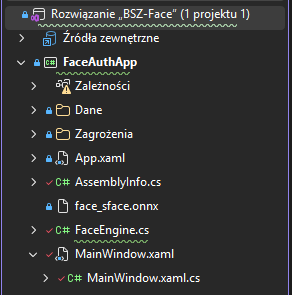
\includegraphics[width=0.45\textwidth]{img/architektura/drzewo_projektu.png}
    \captionof{figure}{Drzewo projektu w środowisku Visual Studio. Widoczny podział na kod widoków (MainWindow.xaml), silnik AI (FaceEngine.cs) oraz wyeksportowany, wstępnie wytrenowany model sieci (face\_sface.onnx).}
\end{center}
